The parallelization strategy we have chosen for this project is \emph{Root-Root parallelization}.
\emph{Root parallelization} consists in giving the tree that we want to develop to every thread, letting them develop it randomly without any communication with the environment during a certain amount of time, and then merging the results of each tree.
This method has the great benefit of minimizing the communication between the actors (the threads or the machines).
That is because they only communicate at the beginning and at the end of the algorithm, without needing any further synchronization.
The \textit{Root Parallelization} is depicted in figure \ref{fig:root}.

\begin{figure}[!ht] 
\centerline{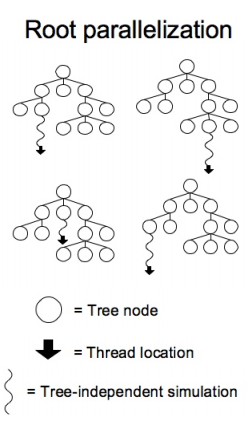
\includegraphics[scale=0.5]{Parallelisation/Strategy/Img/root.png}}
   \caption{Overview of \emph{Root Parallelization} \cite{parallel_comp}}
\label{fig:root}
\end{figure}

\emph{Root-Root parallelization} consists in applying this strategy on two levels : on threads and on machines.
For this we have chosen a master-slave approach, with one master machine collecting the results of every other machine once they are done with their processing.
The same structure will be repeated locally on each machine, with one master thread collecting the results of the other threads.